% !TeX encoding = UTF-8
% !TeX spellcheck = en_US
% !TeX TXS-program:bibliography = biber -l zh__pinyin --output-safechars %
%% !TeX TS-program = lualatex
%%% LuaLaTeX is required for `tikz-feynman`

\documentclass[a4paper,10pt]{article}

\newcommand{\hwNumber}{4}

% to be `\input` in subfolders,
% ... therefore the path should be relative to subfolders.

\usepackage[UTF8
	,heading=false
	,scheme=plain % English Document
]{ctex}

\input{../.modules/basics/macros.tex}
\input{../.modules/preamble_base.tex}
\input{../.modules/preamble_notes.tex}

\newcommand{\normorder}[1]{
	{\mathopen {:}}{\tinyhskip #1\tinyhskip}{\mathclose {:}}
}

\usepackage{simpler-wick}

\newcommand{\tinyhskip}{{\hskip .1em}}
\newcommand{\mat}[1]{\pqty\Big{
	\footnotesize
	\hspace{-.2em}
		\begin{array}{cc}
			#1
		\end{array}
	\hspace{-.2em}
}}

% Settings
\counterwithout{equation}{section}
\mathtoolsset{showonlyrefs=false}
%\DeclareTextFontCommand{\textbf}{\sffamily}
\renewcommand{\midquote}{\quad}

% Spacing
\geometry{footnotesep=2\baselineskip} % pre footnote split
\setlength{\parskip}{.5\baselineskip}
\renewcommand{\baselinestretch}{1.15}

%Title
	\posttitle{
		\hfill\Large\ccbyncsajp
		\par\end{flushleft}%
		\vspace*{-.7ex}\hrule%
	}
	\preauthor{\vspace{-1.5ex}%
		\flushleft\itshape%
	}
	\postauthor{\hfill}
	\predate{\noindent\ttfamily Compiled @ }
	\postdate{\vspace{.5ex}}

	\title{String Theory \textnumero\hwNumber}
	\author{\signature Bryan}
	\date{\today}

% List
	\setlist*{
		listparindent=\parindent
		,labelindent=\parindent
		,parsep=\parskip
		,itemsep=1.2\parskip
	}
	\setlist*[enumerate,1]{
		align=left
		,label=\fbox{\textbf{\arabic*}}
		,itemsep=.5\baselineskip
	}

\input{../.modules/basics/biblatex.tex}

%%% ID: sensitive, do NOT publish!
%\InputIfFileExists{../id.tex}{}{}

\usepackage{cancel}

\begin{document}
\maketitle
\pagestyle{headings}
\pagenumbering{arabic}
\thispagestyle{empty}

	\begin{enumerate}
	\item \textbf{Stringy Physics!}
	\begin{gather}
		T(z)
		= - \frac{1}{\alpha'}\,
			\normorder{\pd X^\mu \pd X_\mu}\,,\quad
		\tilde{T}(\bar{z})
		= - \frac{1}{\alpha'}\,
			\normorder{\pdbar X^\mu \pdbar X_\mu}\,,
	\\[.5ex]
		V_k = \normorder{
				e^{ik\cdot X(z,\bar{z})}
			}\,,\quad
		G_{e,k} = e_{\mu\nu}\,\normorder{
				\pd X^\mu_z\,
				\pdbar X^\nu_{\bar{z}}\,
				e^{ik\cdot X(z,\bar{z})}
			}\,,
	\end{gather}
	We sometimes use subscripts like $
		\pd X^\mu_z
	$ to denote variable dependence to avoid clutter. 
	
	\begin{enumerate}
	\item The weight of a primary operator is given by its OPE with $T$ and $\tilde{T}$. For exponential operators, there is a neat formula for cross contractions\footnote{
		Reference: \textit{Polchinski}, and \https{physics.stackexchange.com/a/389193}. 
	}:
	\begin{equation}
	\begin{aligned}
		T(z)\,V_k(w,\bar{w})
		&= \exp \Bqty{
			\int \dd[2]{z'} 
			\int \dd[2]{w'}
				\wick{
					\c X^\mu_{z'}
					\c X^\nu_{w'}
				}
				\fdv{X^\mu_{z'}}
				\fdv{X^\nu_{w'}}
			}\,
			\normorder{T_z\,e^{ik\cdot X_w}} \\
		&= \exp \Bqty{
			\int \dd[2]{z'}
				\wick{
					\c X^\mu_{z'}
					\c X^\nu_{w}
				}
				\fdv{X^\mu_{z'}}
				\,ik_\nu
			}\,
			\normorder{T_z\,e^{ik\cdot X_w}} \\
		&= \normorder{
			\Bqty{
				\exp \pqty{
					ik_\nu \! \int \dd[2]{z'}
						\wick{
							\c X^\mu_{z'}
							\c X^\nu_{w}
						}
						\fdv{X^\mu_{z'}}
				}\,T_z
			}\,e^{ik\cdot X_w}
		} \\
		&\sim -\frac{1}{\alpha'}\,
			\normorder{
				\Bqty{
					2 \pdd{z} \pqty\big{
						ik_\sigma
						\wick{
							\c X^\mu_{z}
							\c X^\sigma_{w}
						}
					}\, \pdd{z} X_\mu
					+ \pdd{z} \pqty\big{
							ik_\rho
							\wick{
								\c X^\mu_{z}
								\c X^\rho_{w}
							}
						}\,
						\pdd{z} \pqty\big{
							ik_\sigma
							\wick{
								\c X_{z,\mu}
								\c X^\sigma_{w}
							}
						}
				}\,e^{ik\cdot X_w}
			} \\
		&\sim -\frac{1}{\alpha'}\,
			\normorder{
				\Bqty{
					2\,\pqty{
						-\frac{\alpha'}{2}
						\frac{ik^\mu}{z - w}
					}\, \pdd{z} X_\mu
					+ \pqty{
						-\frac{\alpha'}{2}
						\frac{ik^\mu}{z - w}
					} \pqty{
						-\frac{\alpha'}{2}
						\frac{ik_\mu}{z - w}
					}
				}\,e^{ik\cdot X_w}
			} \\
		&\sim
			\frac{\alpha'k^2}{4}
				\frac{V_k(w,\bar{w})}{(z - w)^2}
			+ \frac{\pd V_k(w,\bar{w})}{z - w}
	\end{aligned}
	\end{equation}
	Here we've used the result that $
		ik_\sigma
		\wick{
			\c X^\mu_{z}
			\c X^\sigma_{w}
		}
		= ik^\mu (-\frac{\alpha'}{2})
			\ln \abs{z-w}^2
	$. We see that $V_k$ is a primary of weight $(1,1)$ iff.~$
		\frac{\alpha'k^2}{4}
		= 1
	$, or $
		m^2 = -k^2 = -\frac{4}{\alpha'}
	$. This is the mass shell condition for the closed string tachyon (at level 0). On the other hand,
	\begin{gather}
		G_{e,k}
		= e_{\mu\nu} G^{\mu\nu}_k,\\[1ex]
	\begin{aligned}
		T(z)\,G^{\mu\nu}_k(0)
		&\sim \normorder{\wick{
				\c T_z\,
				\pd \c X^\mu_0\,
				\pdbar X^\nu_0\,
				e^{ik\cdot X_0}
			}}
			+ \cancel{\normorder{\wick{
				\c T_z\,
				\pd X^\mu_0\,
				\pdbar \c X^\nu_0\,
				e^{ik\cdot X_0}
			}}}
			+ \normorder{\wick{
				\c T_z\,
				\pd X^\mu_0\,
				\pdbar X^\nu_0\,
				\c e^{ik\cdot X_0}
			}}
			\\ &\qquad
			+ \cancel{\normorder{\wick{
				\bcontraction[1.1ex]{}{T}{_z\,\pd}{X}
				\c T_z\,
				\pd X^\mu_0\,
				\pdbar \c X^\nu_0\,
				e^{ik\cdot X_0}
			}}}
			+ \normorder{\wick{
				\bcontraction[1.1ex]{}{T}{_z\,\pd}{X}
				\c T_z\,
				\pd X^\mu_0\,
				\pdbar X^\nu_0\,
				\c e^{ik\cdot X_0}
			}}
		\\
		&\sim \pqty{
				\frac{1}{z^2}\, G^{\mu\nu}_k(0)
				+ \frac{1}{z}\, \normorder{
					\pd^2 X^\mu_0\,
					\pdbar X^\nu_0\,
					e^{ik\cdot X_0}
				}
			}
			+ \pqty{
				\frac{\alpha'k^2}{4}
				\frac{1}{z^2}\, G^{\mu\nu}_k(0)
				+ \frac{1}{z}\, \normorder{
					\pd X^\mu_0\,
					\pdbar X^\nu_0\,
					\pd\,e^{ik\cdot X_0}
				}
			}
			\\ &\qquad
			- \frac{2}{\alpha'}
				\pqty{
					-\frac{\alpha'}{2}
					\eta^{\sigma\mu}
					\frac{1}{z^2}
				} \pqty{
					-\frac{\alpha'}{2}
					\frac{ik_\sigma}{z}
				}\, \normorder{
					\pdbar X^\nu_0\,
					e^{ik\cdot X_0}
				}
		\\[1ex]
		&\sim
			ik^\mu\,\normorder{
					\pdbar X^\nu_0\,
					e^{ik\cdot X_0}
				}\,
				\pqty{-\frac{\alpha'}{2}}
				\frac{1}{z^3}
			+ \pqty{
					1 + \frac{\alpha'k^2}{4}
				}\, \frac{G^{\mu\nu}_k(0)}{z^2}
			+ \frac{\pd G^{\mu\nu}_k(0)}{z},
		\\[-1.25\baselineskip]
	\end{aligned}\\[.8\baselineskip]
		\tilde{T}(\bar{z})\,G^{\mu\nu}_k(0)
		\sim
			ik^\nu\,\normorder{
					\pd X^\mu_0\,
					e^{ik\cdot X_0}
				}\,
				\pqty{-\frac{\alpha'}{2}}
				\frac{1}{\bar{z}^3}
			+ \pqty{
					1 + \frac{\alpha'k^2}{4}
				}\, 
				\frac{G^{\mu\nu}_k(0)}{\bar{z}^2}
			+ \frac{\pd G^{\mu\nu}_k(0)}{\bar{z}},
	\end{gather}
	
	\noindent
	Therefore, $G_{e,k}$ is a primary of weight $(1,1)$ iff.~$
		1 + \frac{\alpha'k^2}{4} = 1
	$ and $
		k^\mu e_{\mu\nu}
		= 0 = k^\nu e_{\mu\nu}
	$. The first equation gives the mass shell condition $
		m^2 = -k^2 = 0
	$ for a massless boson, while the second equation constrains the polarization to be transverse. These are the physical constraints for a massless gauge boson, which is the level 1 excitation for a bosonic closed string. 
	
	\item The form of any primary 3-point function is completely fixed by $\mrm{PSL}(2,\mbb{C})$ invariance\footnote{
		Reference: Blumenhagen, \textit{Introduction to CFT}, and also \textit{Di Francesco et al}. 
	}. In fact, for any holomorphic $\phi_i(z_i)$ with weight $h_i$, by translational invariance, we have:
	\begin{equation}
		\ave{
			\phi_1(z_1)\,
			\phi_2(z_2)\,
			\phi_3(z_3)
		}
		= f(z_{12},z_{23},z_{31}),\quad
		z_{ij} = z_i - z_j,
	\end{equation}
%	Here for simplicity we write $\phi_i(z_i)$ in stead of $\phi_i(z_i,\bar{z}_i)$, but the anti-holomorphic dependence is still implied. 
	Furthermore, scaling invariance requires that $f$ is quasi-homogeneous:
	\begin{gather}
	\begin{aligned}
		z\mapsto z' = \lambda^{-1} z,\quad
		f &\mapsto \ave[\big]{
			\lambda^{h_1} \phi_1(\lambda z_1)\,
			\lambda^{h_2} \phi_2(\lambda z_2)\,
			\lambda^{h_3} \phi_3(\lambda z_3)
		} \\[.5ex]
		&= \lambda^{h_1 + h_2 + h_3} f(
				\lambda z_{12},
				\lambda z_{23},
				\lambda z_{31}
			) \\
		&= f(z_{12},z_{23},z_{31}),
	\end{aligned}
	\\[1ex]
		f = \!\! \sum_{
				a + b + c = \sum_i \! h_i
			} f_{abc}
		= \!\! \sum_{
				a + b + c = \sum_i \! h_i
			}
			\frac{C_{abc}}{
				z_{12}^a
				z_{23}^b
				z_{31}^c
			}
	\end{gather}
	
	On the other hand, for special conformal transformation\footnote{
		See \textit{Di Francesco et al}, and also \https{github.com/davidsd/ph229}. 
	} $
		\frac{1}{\bar{z}}
		\mapsto \frac{1}{\bar{z}'}
		= \frac{1}{\bar{z}} + a
	$, we have:
	\begin{gather}
		z\ \longmapsto\ 
		z' = \frac{1}{\frac{1}{z} + \bar{a}}
		= \frac{z}{1 + z\bar{a}}
		= w(z),\quad
		\pdv{z}{z'}
		= \frac{1}{(1 - z\bar{a})^2}
		= \frac{1}{\kappa^2},\quad
		z_{ij}
		= \frac{z'_{ij}}{\kappa_i \kappa_j},\\
		f \ \longmapsto\ %
		f\pqty\Big{
				w^{-1}(z_{12}),
				w^{-1}(z_{23}),
				w^{-1}(z_{31})
			} \frac{1}{
				\kappa_1^{2h_1}
				\kappa_2^{2h_2}
				\kappa_3^{2h_3}
			}
		= f(z_{12},z_{23},z_{31}),\\
		f_{abc}\pqty\Big{
				w^{-1}(z_{12}),
				w^{-1}(z_{23}),
				w^{-1}(z_{31})
			}
		= f_{abc}(z_{12},z_{23},z_{31})\,
			\kappa_1^{c + a}
			\kappa_2^{a + b}
			\kappa_3^{b + c},
	\end{gather}
	We see that $f$ is invariant under special conformal transformation iff.\ $f = f_{abc}$ where:
	\begin{gather}
		c + a = 2h_1,\quad
		a + b = 2h_2,\quad
		b + c = 2h_3,\\
		\text{i.e.}\quad
		a = h_1 + h_2 - h_3,\quad
		b = h_2 + h_3 - h_1,\quad
		c = h_3 + h_1 - h_2,
	\end{gather}
	
	In the above discussions we've restricted $\phi_i$ to be holomorphic; for \textit{spin-less} $
		\phi_i = \phi_i(z,\bar{z}),\ %
		h_i = \tilde{h}_i$, $
		\Delta_i = h_i + \tilde{h}_i
	$, the holomorphic and anti-holomorphic contributions can be nicely combined, and we have:
	\begin{gather}
		f = \frac{C}{
			\abs{z_{12}}^{2a}
			\abs{z_{23}}^{2b}
			\abs{z_{31}}^{2c}
		},\\[1ex]
		2a = \Delta_1 + \Delta_2 - \Delta_3,\quad
		2b = \Delta_2 + \Delta_3 - \Delta_1,\quad
		2c = \Delta_3 + \Delta_1 - \Delta_2,\\
		\ave{
			V_{k_1}(z_1,\bar{z}_1)\,
			V_{k_2}(z_2,\bar{z}_2)\,
			G_{e,k_3}(z_3,\bar{z}_3)
		}
		= \frac{A(k_1,k_2,e)}{
			\abs{z_{12}}^{2}
			\abs{z_{23}}^{2}
			\abs{z_{31}}^{2}
		}
	\end{gather}
	
	\item Following the recipe in (a), we have:
	\begin{equation}
	\begin{aligned}
		V_{k_1}(z_1,\bar{z}_1)\,
		V_{k_2}(z_2,\bar{z}_2)
		&= \normorder{
			\exp \pqty\Big{
				ik_{1,\mu}
				ik_{2,\nu} 
				\wick{
					\c X^\mu_1
					\c X^\nu_2
				}
			}\,
			e^{ik_1\cdot X_1}\,
			e^{ik_2\cdot X_2}
		} \\
		&= \exp \pqty{
				\frac{\alpha'}{2}\,
				k_1\cdot k_2
				\ln \abs{z_{12}}^2
			}\, \normorder{
				e^{ik_1\cdot X_1}\,
				e^{ik_2\cdot X_2}
			} \\
		&= \abs{z_{12}}^{
				\alpha' k_1\cdot k_2
			}\, \normorder{
				e^{ik_1\cdot X_1}\,
				e^{ik_2\cdot X_2}
			}
	\end{aligned}
	\end{equation}
	Apply the on-shell conditions, and we find that:
	\begin{equation}
		\alpha' k_1\cdot k_2
		= \frac{\alpha'}{2} (k_1 + k_2)^2
			- \frac{\alpha'}{2} k_1^2
			- \frac{\alpha'}{2} k_2^2
		= \frac{\alpha'}{2} (-k_3)^2
			- \frac{\alpha'}{2} k_1^2
			- \frac{\alpha'}{2} k_2^2
		= 0 - 2 - 2
		= -4
	\end{equation}
	We are interested in the $\abs{z_{12}}^{-2}$ term in the OPE around $z_2$; it will contribute to the 3-point function discussed in (b). Note that:
	\begin{gather}
	\begin{aligned}
		\normorder{
			e^{ik_1\cdot X_1}\,
			e^{ik_2\cdot X_2}
		}
%		&= \normorder{
%			\exp{ik_1\cdot \pqty{
%				X_2
%				+ z_{12}\,\pd X_2
%				+ \bar{z}_{12}\,\pdbar X_2
%				+ \frac{1}{2}\,z_{12}^2\,
%					\pd^2 X_2
%				+ \frac{1}{2}\,\bar{z}_{12}^2\,
%					\pdbar^2 X_2
%				+ \cdots
%			}}\,
%			e^{ik_2\cdot X_2}
%		} \\
		&= \normorder{
			\pqty{
				\cdots
				+ \frac{1}{2} (ik_1\cdot X_1)^2
				+ \cdots
			}\, e^{ik_2\cdot X_2}
		} \\
		&= \normorder{
			\pqty{
				\cdots
				- \frac{1}{2}\,k_1^\mu k_1^\nu
					\pqty{
						X_2
						+ z_{12}\,\pd X_2
						+ \bar{z}_{12}\,\pdbar X_2
						+ \cdots
					}_\mu 
					\pqty\big{\cdots}_\nu
					+ \cdot
			}\, e^{ik_2\cdot X_2}
		} \\
		&= \normorder{
			\pqty\Big{
				\cdots
				- k_{1,\mu} k_{1,\nu}\,
					\pqty{
						z_{12} \bar{z}_{12}\,
						\pd X^\mu_2\,\pdbar X^\nu_2
					}
				+ \cdots
			}\, e^{ik_2\cdot X_2}
		} \\
		&= \cdots
			- \abs{z_{12}}^2\,
				k_{1,\mu} k_{1,\nu}\,
				G_{k_2}^{\mu\nu}(z_2,\bar{z}_2)
			+ \cdots,
	\end{aligned}\\[1ex]
		V_{k_1}(z_1,\bar{z}_1)\,
		V_{k_2}(z_2,\bar{z}_2)
		= \cdots
			+ \frac{O_{k_1,k_2}(z_2,\bar{z}_2)}{
				\abs{z_{12}}^2
			}
			+ \cdots,\\[.5ex]
		O_{k_1,k_2}(z_2,\bar{z}_2)
		= - k_{1,\rho} k_{1,\sigma}\,
			G_{k_2}^{\rho\sigma}(z_2,\bar{z}_2),
	\end{gather}
	
	Consider the same limit: $z_1 \to z_2$ of the 3-point function, and we find that:
	\begin{equation}
	\begin{aligned}
		z_1 \to z_2,\quad
		\ave{
			V_{k_1}(z_1,\bar{z}_1)\,
			V_{k_2}(z_2,\bar{z}_2)\,
			G_{e,k_3}(z_3,\bar{z}_3)
		}
		&\to \frac{1}{\abs{z_{12}}^2}
			\frac{A(k_1,k_2,e)}{
				\abs{z_{23}}^4
			} \\
		&\sim \frac{1}{\abs{z_{12}}^2}\,
			\ave[\big]{
				O_{k_1,k_2}(z_2,\bar{z}_2)\,
				G_{e,k_3}(z_3,\bar{z}_3)
			},
	\end{aligned}
	\end{equation}
	We see that in the $z_2\to z_3$ limit, we should obtain:
	\begin{equation}
		O_{k_1,k_2}(z_2,\bar{z}_2)\,
		G_{e,k_3}(z_3,\bar{z}_3)
		= \cdots
			+ \frac{A(k_1,k_2,e)}{
				\abs{z_{23}}^4
			}
			+ \cdots,
	\end{equation}
	
	Note that $A(k_1,k_2,e) = A(k_1,k_2,e)\,\idty$ is simply a number; therefore, when finding $A(k_1,k_2,e)$, it is safe to ignore all (non-identity) operator contributions, as they must cancel each other. 
	Similar to (a), we have:
	\begin{equation}
	\begin{aligned}
		G^{\rho\sigma}_{k_2}(z_2, \bar{z}_2)\,
		G^{\mu\nu}_{k_3}(z_3, \bar{z}_3)
		&= \cdots + \normorder{\wick{
				\pd \c1 X^\rho_2\,
				\pdbar \c2 X^\sigma_2\,
				\c3 e^{ik_2\cdot X_2}\,
				\pd \c1 X^\mu_3\,
				\pdbar \c2 X^\nu_3\,
				\c3 e^{ik_3\cdot X_3}
			}}
			\\ & \phantom{{} = \cdots}
			+ \normorder{\wick{
				\pd \c1 X^\rho_2\,
				\pdbar \c2 X^\sigma_2\,
				\c3 e^{ik_2\cdot X_2}\,
				\pd \c1 X^\mu_3\,
				\pdbar \c3 X^\nu_3\,
				\c2 e^{ik_3\cdot X_3}
			}}
			\\ & \phantom{{} = \cdots}
			+ \normorder{\wick{
				\pd \c1 X^\rho_2\,
				\pdbar \c2 X^\sigma_2\,
				\c3 e^{ik_2\cdot X_2}\,
				\pd \c3 X^\mu_3\,
				\pdbar \c2 X^\nu_3\,
				\c1 e^{ik_3\cdot X_3}
			}}
			\\ & \phantom{{} = \cdots}
			+ \normorder{\wick{
				\bcontraction{
					\pd X^\rho_2\,
					\pdbar}{X}{^\sigma_2\,
					e^{ik_2\cdot X_2}\,
					\pd X^\mu_3\,
					\pdbar X^\nu_3\,
				}{e}
				\bcontraction[1.7ex]{
					\pd X^\rho_2\,
					\pdbar X^\sigma_2\,
					}{e}{^{ik_2\cdot X_2}\,
					\pd}{X}
				\pd \c1 X^\rho_2\,
				\pdbar X^\sigma_2\,
				\c2 e^{ik_2\cdot X_2}\,
				\pd X^\mu_3\,
				\pdbar \c2 X^\nu_3\,
				\c1 e^{ik_3\cdot X_3}
			}}
			+ \cdots
	\end{aligned}
	\end{equation}
	\begin{equation*}
	\begin{aligned}
		G^{\rho\sigma}_{k_2}(z_2, \bar{z}_2)\,
		G^{\mu\nu}_{k_3}(z_3, \bar{z}_3)
		&\sim \cdots
			+ \pqty{
					-\frac{\alpha'}{2}
					\eta^{\rho\mu}
					\frac{1}{z^2_{23}}
				}
				\pqty{
					-\frac{\alpha'}{2}
					\eta^{\sigma\nu}
					\frac{1}{\bar{z}^2_{23}}
				}\times 1
			\\ & \phantom{{} = \cdots}
			+ \pqty{
					-\frac{\alpha'}{2}
					\eta^{\rho\mu}
					\frac{1}{z^2_{23}}
				}
				\pqty{
					-\frac{\alpha'}{2}
					\frac{ik^\sigma_3}{\bar{z}_{23}}
				}
				\pqty{
					-\frac{\alpha'}{2}
					\frac{ik^\nu_2}{\bar{z}_{32}}
				}
			+ \pqty\big{
					z\leftrightarrow\bar{z},\ %
					\rho\leftrightarrow\sigma,\ %
					\mu\leftrightarrow\nu
				}
			\\ & \phantom{{} = \cdots}
			+ \pqty{
					-\frac{\alpha'}{2}
					\frac{ik_2^\rho}{{z}_{23}}
				}
				\pqty{
					-\frac{\alpha'}{2}
					\frac{ik_2^\sigma}{\bar{z}_{23}}
				}
				\pqty{
					-\frac{\alpha'}{2}
					\frac{ik_3^\mu}{{z}_{32}}
				}
				\pqty{
					-\frac{\alpha'}{2}
					\frac{ik_3^\nu}{\bar{z}_{32}}
				}
			+ \cdots
%		\\[-1.15\baselineskip]
	\end{aligned}
	\end{equation*}
	\begin{equation}
	\begin{aligned}
		O_{k_1,k_2}(z_2, \bar{z}_2)\,
		G^{\mu\nu}_{k_3}(z_3, \bar{z}_3)
		&\sim \cdots
			- k_1^\mu k_1^\nu \pqty{
					\frac{\alpha'^2}{4}
				} \frac{1}{\abs{z_{23}}^4}
			\\ & \phantom{{} = \cdots}
			- i^2 \pqty{
					k_1^\mu k_2^\nu
					+ k_1^\nu k_2^\mu
				} 
				\pqty{
					\frac{\alpha'}{2}
					(k_1\cdot k_3)
				}
				\pqty{
					\frac{\alpha'^2}{4}
				} \frac{1}{\abs{z_{23}}^4}
			\\ & \phantom{{} = \cdots}
			- i^4 k_3^\mu k_3^\nu \pqty{
					\frac{\alpha'}{2}
					(k_1\cdot k_2)
				}^{\!\!2}
				\pqty{
					\frac{\alpha'^2}{4}
				} \frac{1}{\abs{z_{23}}^4}
			+ \cdots
	\end{aligned}
	\end{equation}
	Again, apply the on-shell conditions, and we find that:
	\begin{gather}
		\frac{\alpha'}{2} k_1\cdot k_2
		= -2,\quad
		\frac{\alpha'}{2} k_1\cdot k_3
		= -\frac{\alpha'}{2} k_1\cdot (k_1 + k_2)
		= -\frac{\alpha'}{2} k_1^2 
			-\frac{\alpha'}{2} k_1\cdot k_2
		= -2 - (-2) = 0,\\[1ex]
%		k_3^\mu k_3^\nu
%		= (k_1 + k_2)^\mu (k_1 + k_2)^\nu
%		= k_1^\mu k_1^\nu + k_2^\mu k_2^\nu
%			+ (k_1^\mu k_2^\mu + k_1^\nu k_2^\mu),
	\begin{aligned}
		A(k_1,k_2,e)
		&= - \frac{\alpha'^2}{4} \pqty\big{
				4 \cancel{
					e_{\mu\nu} k_3^\mu k_3^\nu
				}
				+ e_{\mu\nu} k_1^\mu k_1^\nu
			}
		= - \frac{\alpha'^2}{4}
			e_{\mu\nu} k_1^\mu k_1^\nu \\
		&= - \frac{\alpha'^2}{4}
			e_{\mu\nu} (k_2+k_3)^\mu (k_2+k_3)^\nu
		= - \frac{\alpha'^2}{4}
			e_{\mu\nu} k_2^\mu k_2^\nu \\
		&= - \frac{\alpha'^2}{8}
			e_{\mu\nu} \pqty\big{
				k_1^\mu k_1^\nu
				+ k_2^\mu k_2^\nu
			} \\
		&= - \frac{\alpha'^2}{8}
			e_{\mu\nu} \pqty\Big{
				k_{12}^\mu k_{12}^\nu
				+ \pqty{
					k_1^\mu k_2^\nu
					+ k_1^\nu k_2^\mu
				} 
			},
	\end{aligned}
	\end{gather}
	On the other hand, 
	\begin{gather}
		0 = e_{\mu\nu} k_3^\mu k_3^\nu
		= e_{\mu\nu} (k_1+k_2)^\mu (k_1+k_2)^\nu
		= e_{\mu\nu} \pqty\Big{
				k_{12}^\mu k_{12}^\nu
				+ 2\pqty{
					k_1^\mu k_2^\nu
					+ k_1^\nu k_2^\mu
				} 
			}\\
		A(k_1,k_2,e)
		= - \frac{\alpha'^2}{8}
			e_{\mu\nu} k_{12}^\mu k_{12}^\nu
			\pqty{
				1 - \frac{1}{2}
			}
		= -\frac{\alpha'^2}{16}
			e_{\mu\nu}\, k_{12}^\mu k_{12}^\nu
	\end{gather}
	
	\end{enumerate}
	
	\item \textbf{Strings Scattering Off a Heavy Particle:}
	
	A heavy particle can be modeled by some D0-brane with Neumann boundary condition in the $X_0$ direction\footnote{
		Reference: \arxiv{hep-th/9611214}, \arxiv{hep-th/9605168}, and \textit{Polchinski}. 
	}. The scattering of a closed string tachyon off the heavy particle can then be computed via a disc diagram with two insertions. 
	
	\begin{enumerate}
	\item The conformal Killing group (CKG) of the disc is $\mrm{PSL}(2,\mbb{R})$. It is a 3 dimensional $\mbb{R}$ Lie group, generated by 3 conformal Killing vectors (CKV's); therefore, it is possible to partially fix the positions of the two insertions $V_1,V_2$. On the upper half plane, this can be implemented by putting $z_1,z_2$ on the imaginary axis, with $z_2$ fixed and $z_1$ integrated\footnote{
		Reference: \arxiv{0812.4408}. I would like to thank Lucy Smith for pointing this out. 
	}:
	\begin{equation}
		\mcal{A}
		= g_c^2 e^{-\lambda}
			\int_0^{z_2} \dd{z_1}
			\ave[\Big]{
				\normorder{
					c^x_1
					e^{ik_1\cdot X_1}
				}\,
				\normorder{
					c_2\tilde{c}_2\,
					e^{ik_2\cdot X_2}
				}
			},\quad
		z_2 = i,\quad
		z_1 = iy,\quad y\in[0,1]
	\end{equation}
	Here $c^x$ comes from the CKV that brings $z_1\to iy$. On the disc this can be taken to be a rotation around $z_2$; when mapped to the upper half plane and at around the imaginary axis, this is simply a translation along the $x = \frac{1}{2} \pqty{
		z + \bar{z}
	}$ direction\footnote{
		Reference: \textit{Polchinski}, Chapter 5 \& 6. 
	}, i.e.
	\begin{gather}
		\text{CKV}\colon\ \pdd{x} = \delta^a_x\,\pdd{a}
		\quad\Longrightarrow\quad
		\text{Ghost}\colon\ c^x,\\
		c^x \pdd{x}
		+ c^y \pdd{y}
			= c^z \pdd{z}
			+ c^{\bar{z}} \pdd{\bar{z}},\quad
		c^x = \frac{1}{2} \pqty{
				c^z + c^{\bar{z}}
			}
			= \frac{1}{2} \pqty\big{
				c(z) + \tilde{c}(\bar{z})
			},
	\end{gather}
	The ghost contribution is then:
	\begin{equation}
	\begin{aligned}
		\ave[\big]{
			c^x_1 c_2 \tilde{c}_2
		}
		= \ave[\big]{
			c^x(z_1)\,c(z_2)\,\tilde{c}(\bar{z}_2)
		}
		&= \frac{1}{2} \pqty\Big{
			\ave[\big]{
				c(z_1)\,c(z_2)\,\tilde{c}(\bar{z}_2)
			}
			+ \ave[\big]{
				\tilde{c}(z_1)\,c(z_2)\,
				\tilde{c}(\bar{z}_2)
			}
		} \\[.5ex]
		&= \frac{1}{2} \pqty\Big{
			\ave[\big]{
				c(z_1)\,c(z_2)\,{c}(z'_2)
			}
			+ \ave[\big]{
				{c}(z'_1)\,c(z_2)\,
				{c}(z'_2)
			}
		}, \quad z' = \bar{z}, \\[.5ex]
		&= \frac{C^g_{D^2}}{2} \pqty{
			z_{12} z_{12'} z_{22'}
			+ z_{1'2} z_{1'2'} z_{22'}
		},\quad z_1,z_2\in i\mbb{R}, \\[.2ex]
		&= 2C^g_{D^2} \pqty{
				z_1^2 - z_2^2
			} z_2
	\end{aligned}
	\end{equation}
	
	On the other hand, the $e^{ik_j\cdot X_j}$ contributions is similar to what we've computed in \boxed{1}\,, except that now we should be careful about the boundary conditions of $X^\mu$, which affect the $XX$ contraction in the formulae. For Neumann boundary condition: $\pdd{y} X^0 = 0$, the half-plane propagator from $z'$ can be constructed with an image at $\bar{z}'$ with \textit{the same charge}, i.e.\ we have:
	\begin{equation}
		\wick{ \c X^0_1 \c X^0_2 }
		= - \frac{\alpha'}{2}\, \eta^{00}
				\ln \abs{z_1 - z_2}^2
			- \frac{\alpha'}{2}\, \eta^{00}
				\ln \abs{z_1 - \bar{z}_2}^2
	\end{equation}
	While for Dirichlet boundary $X^i = \mrm{const}$, we can always select the origin so that $X^i = 0$, and in this case the image should have \textit{the opposite charge}, i.e.
	\begin{gather}
		\wick{ \c X^i_1 \c X^j_2 }
		= - \frac{\alpha'}{2}\, \delta^{ij}
				\ln \abs{z_1 - z_2}^2
			+ \frac{\alpha'}{2}\, \delta^{ij}
				\ln \abs{z_1 - \bar{z}_2}^2,
	\\
	\begin{aligned}
		\Longrightarrow\quad
		\normorder{
			e^{ik_1\cdot X_1}
		}\,
		\normorder{
			e^{ik_2\cdot X_2}
		}
		&= \exp \pqty{
				ik_{1,\mu}
				ik_{2,\nu} 
				\wick{
					\c X^\mu_1
					\c X^\nu_2
				}
			}\, \normorder{
				e^{ik_1\cdot X_1}\,
				e^{ik_2\cdot X_2}
			} \\
		&= \abs{z_{12}}^{
				\alpha' k_1\cdot k_2
			}
			\abs{z_{1\bar{2}}}^{
				\alpha' \pqty{
					- k_1^0 k_2^0
					- \vb{k}_1 \cdot \vb{k}_2
				}
			}\, \normorder{
				e^{ik_1\cdot X_1}\,
				e^{ik_2\cdot X_2}
			}
	\end{aligned}
	\end{gather}
	
	Before further calculations, we note that the normal ordering defined here on $D^2$ differs from that on the usual $\mbb{C}^2$; in fact, there are also self-contractions with image charge\footnote{
		This is very much similar to the torus situation, where we also have to consider self-contractions with image charges. More rigorous discussion of $G^r$ is given in \textit{Polchinski}. 
	}:
	\begin{gather}
		\wick{ \c X^\mu(z,\bar{z})\, \c X^\nu(\bar{z},z) }
		= G^{\mu\nu}_r(z,\bar{z})
		= \mp \frac{\alpha'}{2}\, \eta^{\mu\nu}
				\ln \abs{z - \bar{z}}^2,
	\\
		\Longrightarrow\quad
		\ave[\Big]{\normorder{
				e^{ik_1\cdot X_1}\,
				e^{ik_2\cdot X_2}
			}}_{D^2}
		= \ave[\Big]{\normorder{
				e^{ik_1\cdot X_1}\,
				e^{ik_2\cdot X_2}
			}}_{\mbb{C}^2} 
			\exp \pqty{
				\frac{1}{2} \sum_n
				ik_{n,\mu}
				ik_{n,\nu} 
				\wick{
					\c X^\mu_n
					\c X^\nu_n
				}
			},\quad n = 1,2
	\end{gather}
	The $\mquote{\mp}$ sign choice depends on the boundary condition. 
	
	Therefore,
	\begin{equation}
	\begin{aligned}
		\ave[\Big]{
			\normorder{
				e^{ik_1\cdot X_1}
			}\,
			\normorder{
				e^{ik_2\cdot X_2}
			}
		}_{D^2}
		&= \ave[\Big]{\normorder{
				e^{ik_1\cdot X_1}\,
				e^{ik_2\cdot X_2}
			}}_{\mbb{C}^2} 
			\exp \pqty{
				ik_{1,\mu}
				ik_{2,\nu} 
				\wick{
					\c X^\mu_1
					\c X^\nu_2
				}
			}
			\exp \pqty{
				\frac{1}{2} \sum_n
				ik_{n,\mu}
				ik_{n,\nu} 
				\wick{
					\c X^\mu_n
					\c X^\nu_n
				}
			} \\
		&= \ave[\Big]{\normorder{
				e^{ik_1\cdot X_1}\,
				e^{ik_2\cdot X_2}
			}}_{\mbb{C}^2} 
			\exp \pqty{
				\frac{1}{2} \sum_{m,n}
				ik_{m,\mu}
				ik_{n,\nu} 
				\wick{
					\c X^\mu_m
					\c X^\nu_n
				}
			} \\
		&= \ave[\Big]{\normorder{
				e^{ik_1\cdot X_1}\,
				e^{ik_2\cdot X_2}
			}}_{\mbb{C}^2}
			\abs{z_{12}}^{
				\alpha' k_1\cdot k_2
			}
			\abs{z_{1\bar{2}}}^{
				\alpha' \pqty{
					- k_1^0 k_2^0
					- \vb{k}_1 \cdot \vb{k}_2
				}
			}
			\prod_n
				\abs{z_{n\bar{n}}}^{
					\frac{\alpha'}{2} \pqty{
						- (k_n^0)^2
						- \vb{k}_n^2
					}
				}
	\end{aligned}
	\end{equation}
	
	Note that $X^i$ has no zero mode due to the Dirichlet boundary, hence $\int \DD X$ gives a delta function in only the Neumann direction: $
		\delta\pqty{k_1^0 + k_2^0}
	$. Physically, this means that only the energy is conversed; the momentum $k^i$ is not conserved since the heavy D0-brane does not recoil. It is therefore convenient to define these on shell variables:
	\begin{gather}
		s = \omega^2 = (k_1^0)^2 = (k_2^0)^2,\quad
		t = - (\vb{k}_1 + \vb{k}_2)^2
		= - \vb{k}_1^2 - \vb{k}_2^2
			- 2\vb{k}_1 \cdot \vb{k}_2
		= 2 \pqty{
				-\omega^2 - \vb{k}_1 \cdot \vb{k}_2
				- \frac{4}{\alpha'}
			},\\
		\vb{k_1} \cdot \vb{k_2}
		= -\frac{t}{2} - \omega^2
			- \frac{4}{\alpha'},\quad
		k_1 \cdot k_2
		= -\omega(-\omega) + \vb{k_1} \cdot \vb{k_2}
	\end{gather}
	Here we've used the on-shell condition: $
		m^2 = -k^2
		= \omega^2 - \vb{k}^2
		= -\frac{4}{\alpha'}
	$ for tachyons. The previous expressions can then be simplified to:
	\begin{gather}
	\begin{aligned}
		\ave[\Big]{
			\normorder{
				e^{ik_1\cdot X_1}
			}\,
			\normorder{
				e^{ik_2\cdot X_2}
			}
		}_{D^2}
		&= \ave[\Big]{\normorder{
				e^{ik_1\cdot X_1}\,
				e^{ik_2\cdot X_2}
			}}_{\mbb{C}^2}
			\abs{z_{12}}^{
				- \frac{\alpha't}{2} - 4
			}
			\abs{z_{1\bar{2}}}^{
				+ \frac{\alpha't}{2} + 4
				+ 2\alpha'\omega^2
			}
			\prod_n
				\abs{2z_n}^{
					- \alpha'\omega^2 - 2
				} \\
		&= {
				i C^X_{D^2}\,
				2\pi\,\delta\pqty{k_1^0 + k_2^0}
			}\,
			\abs{z_{12}}^{
				- \frac{\alpha't}{2} - 4
			}
			\abs{z_{1\bar{2}}}^{
				+ \frac{\alpha't}{2} + 4
				+ 2\alpha'\omega^2
			}
			\prod_n
				\abs{2z_n}^{
					- \alpha'\omega^2 - 2
				} \\
		&= {
				i C^X_{D^2}\,
				2\pi\,\delta\pqty{k_1^0 + k_2^0}
			}\,
			f\pqty\big{
				\abs{z_{12}},\abs{z_{1\bar{2}}},
				\abs{z_1},\abs{z_2}
			},
	\end{aligned}
	\label{eq:VEV_vertices}\\[2ex]
	\begin{aligned}
		\mcal{A}
		&= g_c^2 \underline{e^{-\lambda}}\cdot {
				i \underline{C^X_{D^2}}\,
				2\pi\,\delta\pqty{k_1^0 + k_2^0}
			}\cdot 2\underline{C^g_{D^2}}\,
			\int_0^{z_2} \dd{z_1}
				\pqty{
					z_1^2 - z_2^2
				} z_2\,
				f\pqty\big{
					\abs{z_{12}},\abs{z_{1\bar{2}}},
					\abs{z_1},\abs{z_2}
				} \\
		&= g_c^2 \underline{C_{D^2}}\,
			2\pi\,\delta\pqty{k_1^0 + k_2^0}
			\cdot 2i
			\int_0^1 i\dd{y}
				\pqty{
					(iy)^2 - i^2
				}\,i\cdot
				f\pqty\big{
					1 - y, 1 + y,
					2y, 2
				} \\
		&= -ig_c^2 C_{D^2}\,
			2\pi\,\delta\pqty{k_1^0 + k_2^0}
			\cdot 2\cdot 2^{-2\alpha'\omega^2 - 4}
			\int_0^1 \dd{y}
				(1 - y^2)\,
				f\pqty\big{
					1 - y, 1 + y,
					y, 1
				},
	\end{aligned}
	\label{eq:Amp_simplified}\\[1ex]
	\begin{aligned}
		\int_0^1 \dd{y}
			(1 - y^2)\,
			f\pqty\big{
				1 - y, 1 + y,
				y, 1
			}
		&= \int_0^1 \dd{y}
				(1 - y)^{
					- \frac{\alpha't}{2} - 4 + 1
				}
				(1 + y)^{
					+ \frac{\alpha't}{2} + 4
					+ 2\alpha'\omega^2 + 1
				}
				y^{
					- \alpha'\omega^2 - 2
				} \\
		&= \int_0^1 \dd{y}
				y^{a-1}
				(1 - y)^{2b-1}
				(1 + y)^{-2a-2b+1},\quad
			y' = \frac{1 - y}{1 + y}, \\
		&= - 2^{1-2a} \int_0^1 \dd{y'}
				(-y')^{2b-1}
				(1 - y'^2)^{a-1} \\
		&= 2^{-2a} \int_0^1 \dd{(y'^2)}
				(y'^2)^{b-1}
				(1 - y'^2)^{a-1} \\
		&= 2^{-2a} B\pqty{
				a = -\alpha'\omega^2 - 1,\,
				b = -\frac{\alpha't}{4} - 1
			} \\
	\end{aligned}
	\label{eq:Beta_integral}
	\end{gather}
	Here $
		B(a,b)
		= \frac{\Gamma(a)\,\Gamma(b)}{\Gamma(a+b)}
	$ is the Euler Beta function. 
	
	Putting everything together, we obtain:
	\begin{gather}
	\begin{aligned}
		\mcal{A}
		&= -ig_c^2 C_{D^2}\,
			2\pi\,\delta\pqty{k_1^0 + k_2^0}
			\cdot \frac{1}{2}\,
			B\pqty{
				-\alpha'\omega^2 - 1,\,
				-\frac{\alpha't}{4} - 1
			} \\
		&= -ig_c^2 C_{D^2}\,
			\pi\,\delta\pqty{k_1^0 + k_2^0}\,
			B\pqty{
				-\alpha'\omega^2 - 1,\,
				-\frac{\alpha't}{4} - 1
			}
	\end{aligned}
	\end{gather}
	In fact $g_c^2 C_{D^2}$ can be further computed by path integral or by comparing physical results. Here we settle for this generic coefficient since it's already enough for our following discussions\footnote{
		And I have run out of time and energy. 
	}. 
	
	\item The Regge limit is found by taking the high energy limit while keeping the momentum transfer fixed; in this case it is achieved by:
	\begin{gather}
		\text{Regge:}\quad
			s = \omega^2 \to\infty,\quad
			t = - (\vb{k}_1 + \vb{k}_2)^2
				\,\ \text{fixed},
	\\[1ex]
	\begin{aligned}
		\mcal{A} \propto
			B\pqty{
				a = -\alpha's - 1,\,
				b = -\frac{\alpha't}{4} - 1
			}
		&= \frac{\Gamma\pqty{
				-\alpha's - 1
			}}{\Gamma\pqty{
				-\alpha's - \frac{\alpha't}{4} - 2
			}}\,
			\Gamma\pqty{-\frac{\alpha't}{4} - 1} \\
		&\sim \Bqty{
				e\pqty{
					\alpha's
					+ \frac{\alpha't}{4} + 3
				}
			}^{\frac{\alpha't}{4} + 1}\,
			\Gamma\pqty{-\frac{\alpha't}{4} - 1} \\[.5ex]
		&\sim \pqty{
				e\alpha'\omega^2
			}^{\frac{\alpha't}{4} + 1}\,
			\Gamma\pqty{-\frac{\alpha't}{4} - 1} \\
		&\sim \pqty{
				\omega^2
			}^{\frac{\alpha't}{4} + 1}\,
			\Gamma\pqty{-\frac{\alpha't}{4} - 1}
	\end{aligned}
	\end{gather}
	Here we've used the Stirling's approximation\footnote{
		For the validity of Stirling's approximation when $z\in\mbb{C},\,\arg z = \pi - \epsilon$ and $\abs{z}\to\infty$, see \wikiref{https://en.wikipedia.org/wiki/Stirling\%27s\_approximation\#Stirling's\_formula\_for\_the\_gamma\_function}{Stirling's formula for the gamma function}. 
	}: $
		\ln \Gamma(z + 1)
		= \ln z!
		\sim z\ln z - z
	$. On the other hand, the hard scattering limit is found by keeping the scattering angle fixed, i.e.
	\begin{gather}
		\text{Hard scattering:}\quad
			s = \omega^2 \to\infty,\quad
			\pqty{t/s} \equiv \lambda\,\ \text{fixed},
	\\[1.5ex]
	\begin{aligned}
		\mcal{A}
		\propto B(a,b)
		= \frac{\Gamma(a)\,\Gamma(b)}{
				\Gamma(a+b)
			}
		&\sim \exp\Bqty{
				-\alpha'\pqty{
					s\ln (\alpha's)
					+ \tfrac{t}{4} \ln \tfrac{\alpha't}{4}
					+ \tfrac{u}{4} \ln \tfrac{\alpha'u}{4}
				}
			},
	\end{aligned}
	\\[1.5ex]
		s = \omega^2 = (k_1^0)^2 = (k_2^0)^2,\quad
		t = - (\vb{k}_1 + \vb{k}_2)^2,\quad
		u = - (\vb{k}_1 - \vb{k}_2)^2,
	\\[.5ex]
		s + \frac{t}{4} + \frac{u}{4} = - \frac{4}{\alpha'},
	\end{gather}
	Here we've introduced an additional $u$ variable, and we see that the result is symmetric under $
		t\leftrightarrow u
	$. We find that under the above limits, the amplitude exhibits similar behaviors as the Veneziano amplitude. 
	
	\item Note that $\Gamma(z)$ has no zeros on $\mbb{C}^2$, therefore the poles of $
		B(a,b) = \frac{\Gamma(a)\,\Gamma(b)}{\Gamma(a+b)}
	$ is given by the poles of $\Gamma(a)$ and $\Gamma(b)$:
	\begin{equation}
		a = -\alpha's - 1 = 0,-1,-2,\,\cdots,\quad
		b = -\frac{\alpha't}{4} - 1 = 0,-1,-2,\,\cdots,
	\end{equation}
	
	The first set of poles gives:
	\begin{equation}
		\omega^2 = -\frac{1}{\alpha'},0,
			\frac{1}{\alpha'},
			\frac{2}{\alpha'},\,\cdots
	\end{equation}
	This is precisely the open string spectrum in $D = 26$. Going back to \eqref{eq:VEV_vertices}\,\textasciitilde\,\eqref{eq:Beta_integral}, we see that they come from the singularities as $y = \abs{z_1}\to 0$ or $\abs{z_{12}}\to 1$, i.e.\ the two insertions are far apart. 
	
	This is the $s$-channel contribution; physically, it means that the closed string is first absorbed by the D0-brane, then it propagates as an intermediate open string on the brane, and is re-emitted in the end. 
	
	The other set of poles gives:
	\begin{equation}
		-t =  (\vb{k}_1 + \vb{k}_2)^2
		= \frac{4}{\alpha'},0,
			\cancel{
				-\frac{4}{\alpha'},
				-\frac{8}{\alpha'},\,\cdots
			}
	\end{equation}
	Only two poles are realistic due to $\vb{k}^2 \ge 0$. This is the $t$-channel contribution, which corresponds to a closed string exchange between the D0-brane and the incoming particle. The above factorization channels are nicely illustrated in the diagram below, borrowed from \arxiv{hep-th/9611214}. 
	\begin{center}
	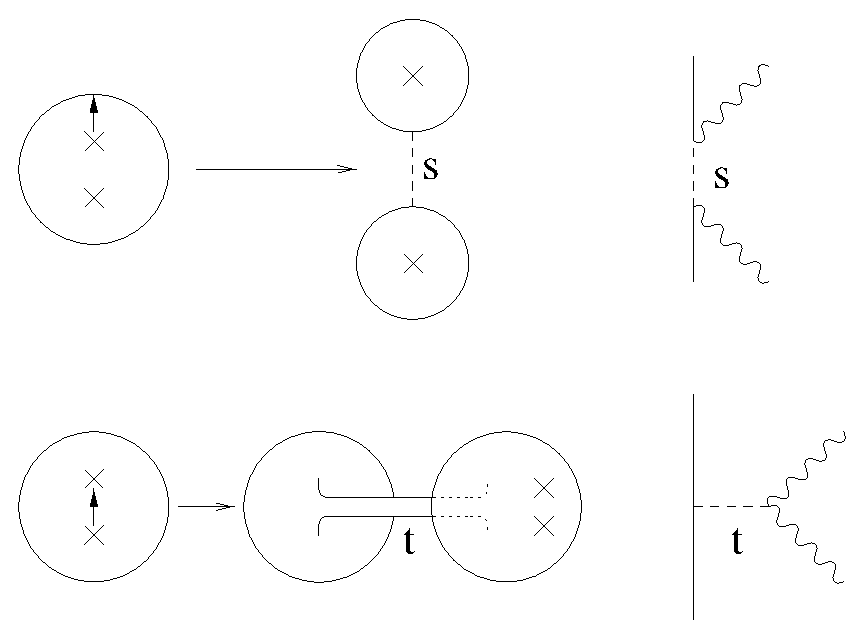
\includegraphics[width=.5\linewidth]{factorize.eps}
	\end{center}
	
	\end{enumerate}
	
	\item \textbf{Compton Scattering Between $U(N)$ Gluons and Adjoint Tachyons:}
	
	Such scattering is captured by a disc diagram with $AATT$ insertions at the boundary; following the same recipe as before, we write down\footnote{
		I would like to thank \textit{谷夏} for help with this problem. 
	}:
	\begin{equation}
	\begin{aligned}
		\mcal{A}
		&= g_o'^2 g_o^2 e^{-\lambda}
			\int \dd{y}
			\ave[\Big]{
				\normorder{
					e_\mu \pdd{y} X^\mu\,
					e^{ik\cdot X}(y)
				}\,
				\normorder{
					c^y_1\,
					e_{1,\nu} \pdd{y} X_1^\nu\,
					e^{ik_1\cdot X_1}
				}\,
				\normorder{
					c^y_2
					e^{ik_2\cdot X_2}
				}\,
				\normorder{
					c^y_3
					e^{ik_2\cdot X_2}
				}
			} 
			\\ & \qquad
			\times\Tr \pqty\big{
				\lambda^a
				\lambda^{a_1}
				\lambda^{a_2}
				\lambda^{a_3}
				\colon \text{in $(y,y_1,y_2,y_3)$ order}
			}
			\\[.8ex] & \quad
			+ \pqty\big{2\leftrightarrow 3}
	\end{aligned}
	\end{equation}
	Where $y_i = y_{1,2,3}$ are fixed while $y_0 = y$ is integrated. 
	Note that for \boxed{2} we use $(x,y)$ to label the points on the upper half plane so that the boundary coordinate is $x = (x,0)$; here in order to match with \textit{Polchinski}, we label the boundary points with $y = (y,0)$ instead. 
	
	We see that $\mcal{A}$ is structurally similar to the 4-point Veneziano amplitude $\mcal{A}_{TTTT}$ and also the 3-point amplitude $\mcal{A}_{TTA}$; by analogy we can evaluate $\mcal{A}$ in a similar fashion\footnote{
		For the $\pd X$ contribution, see \textit{Polchinski}, \arxiv{1403.4553} and \arxiv{1507.02172}. Note that there are contractions between two $\pd X$ fields. 
	}:
	\begin{equation}
	\begin{aligned}
		\mcal{A}
		&= g_o'^2 g_o^2 e^{-\lambda}
			\prod_{i<j}
				\abs{y_{ij}}^{2\alpha'k_i\cdot k_j + 1}\,
			e_{\mu} e_{1,\nu} 
			\\ & \qquad
			\times \int \dd{y}
				\prod_{j}
					\abs{y_{0j}}^{2\alpha'k\cdot k_j}\,
				\Bqty{
					-2\alpha'
						\frac{\eta^{\mu\nu}}{y_{01}^2}
					+ (-2\alpha') \pqty{
						\frac{ik_1^\mu}{y_{01}}
						+ \frac{ik_2^\mu}{y_{02}}
						+ \frac{ik_3^\mu}{y_{03}}
					}
					(-2\alpha') \pqty{
						\frac{ik^\nu}{y_{10}}
						+ \frac{ik_2^\nu}{y_{12}}
						+ \frac{ik_3^\nu}{y_{13}}
					}
				}
			\\[1ex] & \qquad\qquad
			\times
			\Tr\,(\cdots)\,
			iC^X_{D_2} C^g_{D_2}\,(2\pi)^{26}
				\delta^{26}\pqty\big{
					\textstyle\sum_i k_i
				}
			\\[1.8ex] & \quad
			+ \pqty\big{2\leftrightarrow 3}
	\end{aligned}
	\end{equation}
	Notice the doubling due to the boundary contraction $
		\wick{\c X_1^\mu \c X_2^\nu}
		= 2\times \pqty\big{-\frac{\alpha'}{2}}
			\ln y_{12}^2
		= -2\alpha' \ln y_{12}
	$. 
%	We've applied
	Further simplifications can be achieved by using the on-shell and physical conditions for open string states:
	\begin{gather}
		k^2 = k_1^2 = 0,\quad
		e\cdot k = e_1 \cdot k_1 = 0,\quad
		k_{2,3}^2 = \frac{1}{\alpha'} = -m^2,\\
	\begin{aligned}
		s &= -\alpha'(k + k_1)^2 = -2\alpha'k\cdot k_1,\\
		t &= -\alpha'(k + k_2)^2
			= -2\alpha'k\cdot k_2 - 1,\\
		u &= -\alpha'(k + k_3)^2
			= -2\alpha'k\cdot k_3 - 1,
	\end{aligned}
	\\
		s + t + u = -2,\\
%		2\alpha'k_1\cdot (k_2 + k_3)
%		= -2\alpha'k_1\cdot (k_1 + k)
%		= -2\alpha'k_1\cdot k = s, \\
%		e_1\cdot (k_2 + k_3)
%		= -e_1\cdot (k_1 + k)
%		= -e_1\cdot k, \quad
%		e\cdot (k_2 + k_3)
%		= -e\cdot k_1,
		2\alpha' k_1\cdot k_2
		= \alpha'(k_1 + k_2)^2
			- \alpha'k_1^2
			- \alpha'k_2^2
		= \alpha'(k + k_3)^2 - 1
		= - u - 1
		= 2\alpha' k\cdot k_3,\\
		2\alpha' k_1\cdot k_3
		= - t - 1
		= 2\alpha' k\cdot k_2,\\
		2\alpha' k_2\cdot k_3
		= \alpha'(k + k_1)^2 - 2
		= - s - 2,
	\end{gather}
	\vspace{-1\baselineskip}
	\begin{equation}
	\begin{aligned}
		\mcal{A}
		&= ig_o'^2 g_o^2 C_{D^2}\,
			\abs{y_{12}}^{-u}\,
			\abs{y_{13}}^{-t}\,
			\abs{y_{23}}^{-s-2}\,
			e_{\mu} e_{1,\nu} 
			\\[1ex] & \qquad
			\times \int \dd{y}
				\abs{y_{01}}^{-s}
				\abs{y_{02}}^{-t-1}
				\abs{y_{03}}^{-u-1}
				\Bqty{
					\frac{\eta^{\mu\nu}}{y_{01}^2}
					- 2\alpha'
					\pqty{
						\frac{ik_1^\mu}{y_{01}}
						+ \frac{ik_2^\mu}{y_{02}}
						+ \frac{ik_3^\mu}{y_{03}}
					}
					\pqty{
						- \frac{ik^\nu}{y_{01}}
						+ \frac{ik_2^\nu}{y_{12}}
						+ \frac{ik_3^\nu}{y_{13}}
					}
				}
			\\[.8ex] & \qquad\qquad
			\times
			\Tr\,(\cdots)\,
			(-2\alpha') (2\pi)^{26}
				\delta^{26}\pqty\big{
					\textstyle\sum_i k_i
				}
			\\[1ex] & \quad
			+ \pqty\big{2\leftrightarrow 3} 
		\\[1ex]
	\end{aligned}
	\end{equation}
	Fix $y_1 \to \infty, y_2 = 0, y_3 = 1$, and we get:
	\begin{equation}
	\begin{aligned}
		\mcal{A}
		&= ig_o'^2 g_o^2 C_{D^2}\,
%			\prod_{j = 2,3}
			\abs{y_{1}}^{
				- u - t
			}\,
			e_{\mu} e_{1,\nu}
			\\[1ex] & \qquad
			\times \int \dd{y}
				\abs{y_{01}}^{-s}
				\abs{y_{02}}^{-t-1}
				\abs{y_{03}}^{-u-1}
				\Bqty{
					\frac{\eta^{\mu\nu}}{y_{01}^2}
					- 2\alpha'
					\pqty{
						\frac{ik_1^\mu}{y_{01}}
						+ \frac{ik_2^\mu}{y_{02}}
						+ \frac{ik_3^\mu}{y_{03}}
					}
					\pqty{
						- \frac{ik^\nu}{y_{01}}
						+ \frac{ik_2^\nu}{y_{12}}
						+ \frac{ik_3^\nu}{y_{13}}
					}
				}
			\\ & \qquad\qquad
			\times \Tr\,(\cdots)\,\cdots + \cdots
	\end{aligned}
	\end{equation}
	\begin{equation}
	\begin{aligned}
		\mcal{A}
		&= ig_o'^2 g_o^2 C_{D^2}\,
			\\[1ex] & \qquad
			\times \int \dd{y}
				\abs{y_{02}}^{-t-1}
				\abs{y_{03}}^{-u-1}
				\abs{\frac{y_1^{s+2}}{y_{01}^s}}\,
				\Bqty{
					\frac{e\cdot e_1}{y_{01}^2}
					- 2\alpha' e_\mu \pqty{
						\frac{ik_1^\mu}{y_{01}}
						+ \frac{ik_2^\mu}{y_{02}}
						+ \frac{ik_3^\mu}{y_{03}}
					}
					e_{1,\nu} \pqty{
						- \frac{ik^\nu}{y_{01}}
						+ \frac{ik_2^\nu}{y_{12}}
						+ \frac{ik_3^\nu}{y_{13}}
					}
			}
			\\ & \qquad\qquad
			\times \Tr\,(\cdots)\,\cdots + \cdots
	\\[1ex]
		&= ig_o'^2 g_o^2 C_{D^2}\,
			\int \dd{y} \Bqty\Big{
				(e\cdot e_1)\,f(t,u)
				- 2\alpha' g(t,u)
			} \times \cdots + \cdots
	\end{aligned}
	\end{equation}
	Note that the definition of $f(t,u)$ and $g(t,u)$ contains the $\Tr\,(\cdots)$ factor. 
	
	The limit $y_1\to\infty$ should be treated with care. In fact, the integral along the boundary splits into three ranges\footnote{
		Reference: \textit{Polchinski}'s discussion of $\mcal{A}_{TTTT}$. 
	}:
	\begin{equation}
		\int \dd{y}
		= \Bqty{\int_{y_1\to -\infty}^{y_3 = 0}
			+ \int_{y_2 = 0}^{y_3 = 1}
			+ \int_{y_3 = 1}^{y_1\to +\infty}}\dd{y}
	\end{equation}
	Notice the difference of $y_1\to\pm\infty$; this is due to the $S^1$ topology of the boundary. Therefore,
	\begin{gather}
		\int \dd{y} f(t,u)
		= \int \dd{y}
			\abs{y_{02}}^{-t-1}
			\abs{y_{03}}^{-u-1}
			\abs{\frac{y_1}{y_{01}}}^{s+2}
			\Tr\,(\cdots),\\
		\Tr \pqty\big{
			\lambda^a
			\lambda^{a_1}
			\lambda^{a_2}
			\lambda^{a_3}
		}\equiv T_{0123},
	\\[2ex]
	\begin{gathered}
		\int_{y_1\to -\infty}^{y_2 = 0} \dd{y} f(t,u)
		= \int_{y_1\to -\infty}^0 \dd{y}
			(1-y)^{-t-1}
			(-y)^{-u-1}
			\pqty{\frac{-y_1}{y - y_1}}^{s+2}\!\!
			T_{1023}
		= T_{1023} B(-u,-s-1),\\
		\int_{y_3 = 1}^{y_1\to +\infty} \dd{y} f(t,u)
		= \int_{1}^{y_1\to +\infty} \dd{y}
			(y-1)^{-t-1}
			y^{-u-1}
			\pqty{\frac{y_1}{y_1 - y}}^{s+2}\!\!
			T_{1230}
		= T_{1230} B(-t,-s-1),\\
		\int_{y_3 = 0}^{y_2 = 1} \dd{y} f(t,u)
		= \int_0^1 \dd{y}
			(1-y)^{-t-1}
			y^{-u-1}
			t_{1203}
		= T_{1203} B(-t,-u),
	\end{gathered}
	\\[0ex]
		\int \dd{y} f(t,u)
		= T_{1203} B(-t,-u)
			+ T_{1230} B(-t,-s-1)
			+ T_{1023} B(-u,-s-1)
	\end{gather}
	Under $2\leftrightarrow 3$, we have $t\leftrightarrow u$; therefore,
	\begin{equation}
	\begin{aligned}
		\int \dd{y} f(t,u)
			+ \pqty\big{2\leftrightarrow 3}
		&= \pqty{T_{1203} + T_{1302}}\, B(-t,-u)
			\\[-1ex] &\qquad
			+ \pqty{T_{1230} + T_{1032}}\, B(-t,-s-1)
			\\ &\qquad
			+ \pqty{T_{1023} + T_{1320}}\, B(-u,-s-1)
	\\[1ex]
		&\equiv \alpha B(-t,-u)
			+ \beta B(-t,-s-1)
			+ \gamma B(-u,-s-1)
	\end{aligned}
	\end{equation}
	The $g(t,u)$ factor can be computed in a similar manner. In the end we have\footnote{
		Reference: \arxiv{0801.3358}. 
	}:
	\begin{gather}
	\begin{aligned}
		\mcal{A}
		&= ig_o'^2 g_o^2 C_{D^2}\,
			(2\pi)^{26}
			\delta^{26}\pqty\big{
				\textstyle\sum_i k_i
			}
		\\[1ex] & \qquad
			\times(-2\alpha')\,\Big\{
				(e_0\cdot e_1)\,\pqty\big{
					\alpha B(-t,-u)
					+ \beta B(-t,-s-1)
					+ \gamma B(-u,-s-1)
				}
		\\ & \qquad\qquad\qquad
				+ (-2\alpha')
				(e_0\cdot k_2) (e_1\cdot k_3)\,
				\pqty\big{
					\alpha B(-t,-u)
					- \beta B(-t,-s-1)
					- \gamma B(-u,-s-1)
				} + \pqty\big{2\leftrightarrow 3}
			\Big\} \\[1ex]
	\end{aligned}
	\end{gather}
	
	\end{enumerate}


\printbibliography[%
%	title = {参考文献} %
	,heading = bibintoc
]
\end{document}
